\section{Performance Evaluation}

In this section, we perform a performance evaluation of our proposal mechanism using a Netronome SmartNIC. We start describing our environment setup, followed by the discussion of results.

\subsection{Setup}

Our environment setup consists of three high-end servers. Each server has an Intel Xeon 4214R processor with 32 GB RAM. One server is our Device Under Test (DUT) -- i.e., the server in which P4 programs are loaded -- and the others are our traffic generator. All servers have a Netronome SmartNIC Agilio CX 10 Gbit/s network device with two network interfaces, which are physically connected. 
%
We use MoonGen\cite{moongen} as our DPDK\footnote{\url{https://www.dpdk.org/}} traffic generator. We instruct MoonGen using the Netronome Packet Generator\footnote{\url{https://github.com/emmericp/MoonGen/tree/master/examples/netronome-packetgen}}. In our experiments, we send IPv4 packets at line rate (i.e., 10Gbit/s) with random source and destination prefixes. All experiments were run at least 30 times to ensure a confidence level higher than 90\%.


%\subsection{Metrics}
%In our evaluation, we aim to measure the performance of P4 programs with respect to the achieved throughput and latency, and identify existing hardware limitations. We evaluate the impact on those metrics regarding (\textit{i}) the number of operations on registers, (\textit{ii}) the number of access to match+action tables, (\textit{iii}) the number of packet recirculation, (\textit{iv}) the number of applied cryptography functions, and (\textit{v}) the number of performed arithmetic operations. 
%
%To evaluate these metrics, we automatically generate P4 codes with the properties to be analyzed. All P4 codes have at least one match+action table used to perform IP forwarding between physical ports. After generating the P4 source codes, we compiled them using the Netronome compiler and loaded the generated firmware into the physical SmartNIC. Then, we pump network traffic with MoonGen and collect the obtained throughput and latency. To measure data plane latency (i.e., the amount of time a packet stays on PDP), all P4 programs have at least one register which keeps that information (i.e., the difference between the ingress and egress timestamps). During our experiments, we read that register data using the Netronome CLI. The obtained throughput (measured in packets per second) is obtained directly from MoonGen. In order to foster reproducibility, our experimental codes are public available\footnote{\url{https://github.com/mcluizelli/performanceSmartNIC}}. It is important to note that other SmartNICs and compilers can be easily adapted to our experimental codes.

\subsection{Results}

\subsubsection{The cost of reading and writing at multiple registers}

We start by analyzing the cost of performing multiple register operations in the P4 pipeline. Register operations are one of the main building blocks of recent P4 applications (e.g., \cite{hhh-sigcomm,WANG201998, xiong2019switches}). In the experiments, we varied the number of register operations performed sequentially by the P4 program from $10$ to $200$ registers while varying the register width from $32$- to $512$-bit words. We consider that registers are placed in the ingress pipeline and are either read, write, or read \& write. Our goal is to quantify the impact on throughput and latency, as well as to quantify the existing limitation of the current architecture. Figure \ref{fig1} illustrates the measured throughput (in packets per second) and latency (in nanoseconds).\\

\begin{figure}[!tb]
\centering
\subfigure[Measured throughput for different register operations (packet size 64B).]{
            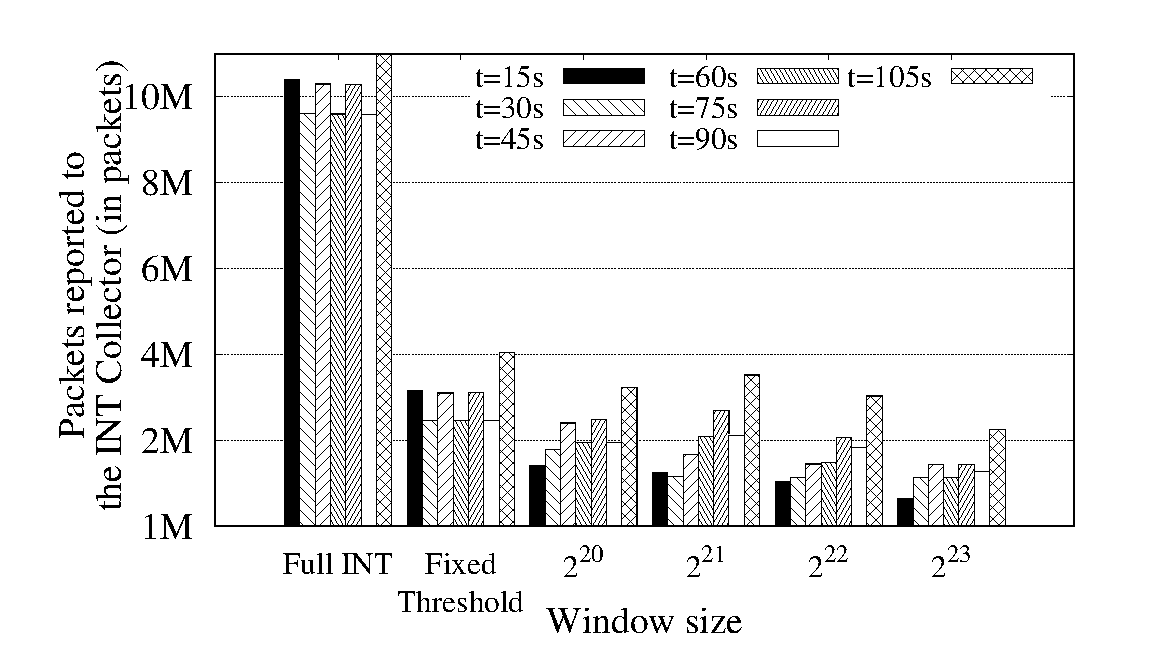
\includegraphics[scale=0.26]{results/g1a.eps}
            \label{fig1-a}
        }
\subfigure[Measured latency for different register operations (packet size 64B).]{
            \includegraphics[scale=0.26]{results/g1b.eps}
            \label{fig1-b}
        }
        \subfigure[Measured throughput for different packet  sizes.]{
            \includegraphics[scale=0.26]{results/g2a.eps}
            \label{fig1-c}
        }
\subfigure[Measured latency for different packet sizes.]{
            \includegraphics[scale=0.26]{results/g2b.eps}
            \label{fig1-d}
        }
        \subfigure[Measured throughput for different register width.]{
            \includegraphics[scale=0.26]{results/g3a.eps}
            \label{fig1-e}
        }
\subfigure[Measured latency for different register width.]{
            \includegraphics[scale=0.26]{results/g3b.eps}
            \label{fig1-f}
        }
        \caption{Measured throughput and latency for register operations.}
        \label{fig1}
\end{figure}

%(Packet size = 64 / register width = 32).
\noindent \textbf{Packet intense line-rate network throughput.} Figures~\ref{fig1-a} and \ref{fig1-b} depict the measured throughput and latency, respectively, for small packets (64 Bytes) and register width of 32 bits. As the number of registers increases (and consequently the number of P4 instructions), there is a sharp performance degradation on observed throughput and latency. The line rate for 10 Gbit/s (i.e., 14.88 million packets per second -- Mpps) can be sustained for reading operations to only 10 registers (Figure~\ref{fig1-a}). Even with 10 registers, the bandwidth degradation for writing operations is 30\% (and it reaches 50\% for read \& write) -- as they demand more micro engine cycles to be performed. After, we observe a linear decrease of up to 87\% (i.e., 2 Mpps) considering 200 registers. In Figure \ref{fig1-b}, the latency increases linearly as the number of operations performed by each processed packet in the pipeline. For a small number of registers (i.e., 10), there is an acceptable overhead of 8650ns (reading), 20296ns (writing), and 35839ns (both operations). However, this overhead can be as high as 0.12 and 0.24 milliseconds for 50 and 200 registers, respectively.
\\

\noindent \textbf{Line rate network throughput for different packet sizes.} Figures~\ref{fig1-c} and \ref{fig1-d} depict the measured throughput and latency, respectively, for different packet sizes (from 64B to 1500B). We fixed the register width to 32 bits and the register operation to read \& write (as it is the most resource-consuming one). Observe that the larger the packet size (and, consequently, the less the number of packets per second to achieve 10Gbit/s), the more register operations can be sustained at line rate. For instance, to 512B-size packets, the line rate throughput can be sustained up to 60 registers being read and write (2Mppps). For 1024B-size packets and higher, there is no throughput degradation -- even for 200 registers. Although there is no throughput degradation, Figure \ref{fig1-d} illustrates that per-packet latency increases substantially. For instance, for 1500B-size packet, the latency increases up to 3X (from 7983ns to 22172ns), while for small packet sizes (and, consequently, higher packet throughput), this latency overhead can be as high as 0.25 millisecond per packet (i.e., a 34X increase).\\




\noindent \textbf{Line rate network throughput for different register width.} Figure~\ref{fig1-e} and Figure \ref{fig1-f} illustrate the throughput and the latency for a varying width of registers. We fixed the packet size to 64B and the operation to read -- as the goal is to quantify the performance degradation with respect to the achieved line rate. As one can observe, the line-rate operation is kept for a register width of up to 128 bits (and 10 registers). Larger register width demands more cycles to fetch the data from memory. As discussed in Section II, Netronome SmartNIC follows a 32-bit architecture. Therefore, any register width wider than that requires extra cycles to be fetched. In addition to that, it is important to mention the memory hierarchy. The more register is needed, the more external memories are used -- which directly affects the time to fetch data. \\

\noindent \textbf{Current limitations.} \emph{Is there any limitation on operating registers in a SmartNIC?} In our experiments, we were able to define at most six arrays of 32-bit registers, each having 130M positions. This limitation is due to the amount of memory available on the board (see Section II). Although we could instantiate such a large number of registers, we could not access all of them in a single pipeline pass because micro engines have a limited code space to store the instruction set (i.e., at most 8K instruction). Differently from traditional languages, P4 does not have go-to primitives, and therefore all instructions are defined at compiling time. For that reason, we were able to operate at most 200 registers in a single P4 program (considering that our P4 program has also other instructions to perform the forwarding). 


%Netronome supports code sharing between micro engines. However, in practice, this has not increased the amount of instructions supported in our experiments.

\subsubsection{Impact of packet recirculation}

\begin{figure}[!tb]
\centering
\subfigure[Measured throughput.]{
            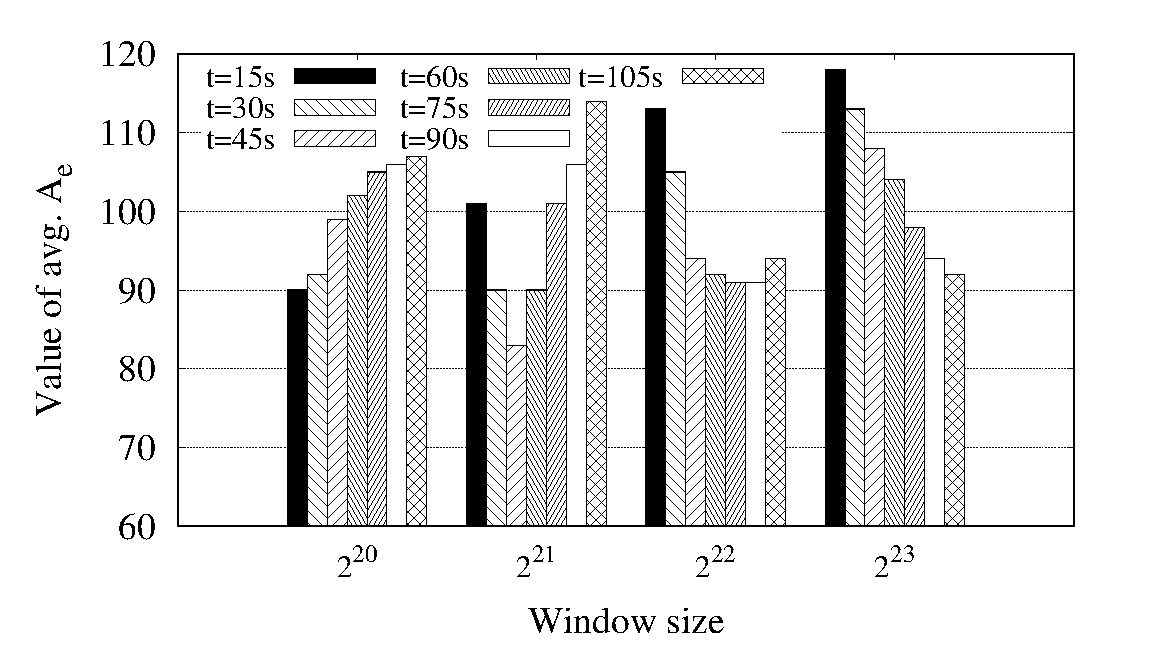
\includegraphics[scale=0.25]{results/g4a.eps}
            \label{fig2-a}
        }
\subfigure[Measured latency.]{
            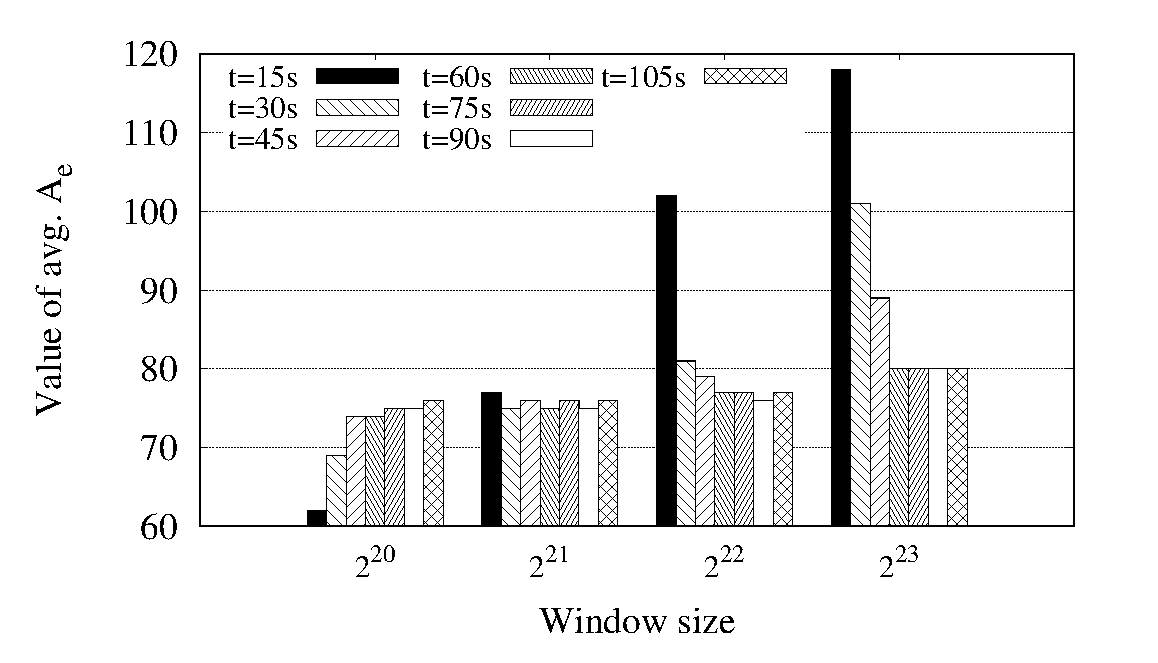
\includegraphics[scale=0.25]{results/g4b.eps}
            \label{fig2-b}
        }
        \caption{Analysing the effect of packet recirculation in the P4 pipeline.}
        \label{fig2}
\end{figure}

Next, we evaluate the impact of performing packet recirculation in the P4 pipeline. As previously mentioned, the P4 language does not support iteration-based structures, and therefore, packet recirculation has been used as a way to circumvent such limitations. In short, packet recirculation consists of sending a packet back to the ingress pipeline after processing it (and therefore, mimic a loop-based structure). In the experiments, we varied the number of packet recirculation made (from 0 to 50) in each packet while varying the packet size (from 64B to 1500B). We consider that our P4 program is just forwarding network traffic from physical interfaces. Figure \ref{fig2} illustrates the measured throughput and latency. 

Figure~\ref{fig2-a} illustrates the throughput behavior as the number of packet recirculations increases (it decreases in a super-linear manner). For small-packet network traffic, we observe that fewer packet recirculations are sustained at line rate (e.g., three packet recirculations for 128B size packets). In contrast, for larger packets (e.g., 1024B), it can maintain line rate even for up to two dozen packet recirculations. As the packets are recirculated, more packets are being pushed into the data plane -- which enqueue them, and eventually dropped occurs (reducing throughput). In turn, Figure~\ref{fig2-b} depicts the observed latency. As one can observe, there is a non-negligible increase in latency as packets recirculate. For instance, even for large packets (e.g., 1500B) -- in which we observe little or no throughput degradation, the per-packet latency doubles on performing just $3$ packet recirculations (from 5610ns to 10688ns). This overhead is even sharper as the number of recirculations increases. For example, there is a 6x latency increase (32762ns) for doing 10 recirculations, and an 80x latency increase (450062ns) for 50 recirculations. As one can observe, this overhead is even greater for small packets.

\noindent \textbf{Current limitations.} In our experiments, we observe that the Netronome architecture does not allow for recirculating custom-made metadata structure. This limits substantially the ability to write complex P4 programs -- especially the ones using packet recirculation to circumvent the lack of iteration-based structure.


\subsubsection{Impact of using multiple tables}

We  evaluate  the  impact  of  using multiple match-action tables. Unlike traditional forwarding devices that use match+action tables exclusively for routing (i.e., to look up network addresses), the P4 language has opened up new possibilities for this construction type. For instance, Xiong et al.~\cite{xiong2019switches} have used multiple tables to implement data plane clustering approaches (e.g., k-means with a table per cluster). Similar to the work conducted by Harkous et al.~\cite{harkous2019towards}, we also observe that the performance of P4 programs is not affected by the size of tables -- as a hash-based data structure implements them. Usually, large match+action tables are already placed on larger and slow memories (e.g., DRAM). Here, instead, we aim at analyzing the impact of using multiple match+action tables at different stages of the pipeline. In the experiments, we varied the number of existing tables in our P4 programs (from 1 to 10), and we ensure that every packet is always matched sequentially on all tables. An action is invoked to read a single 32-bit data from the table and store it in a metadata structure on a packet matching. We varied the packet size (from 64B to 1500B) and the number of tables per pipeline (either on the ingress or egress pipeline). Figure \ref{fig3} illustrates the measured throughput and latency. 

Figure \ref{fig3-a} illustrates the measured throughput for an increasing number of match+action tables. As observed, the throughput for 64B packets (most packet intensive network traffic) is almost negligible for up to 5 match+action tables (i.e., it keeps the line rate). However, we observe an abrupt decay after 5 tables, followed by a constant throughput behavior (up to 10). In the Netronome architecture, a P4 program can only have 5 tables in each pipeline (ingress/egress). Therefore, tables $1-5$ are located in the ingress pipeline, while $6-10$ in the egress. As all the memory is statically allocated for a P4 program, the Netronome compiler tends to use faster, closer available memory to micro engines to allocate ingress tables. Even when defining tables only in the egress pipeline, the compiler tends not to use faster memory. We empirically show this behavior in Figure \ref{fig3-c}. We incrementally place 5 tables either in the ingress or egress pipeline. We observe that the ingress pipeline is always faster to use available tables (w.r.t. latency) -- even in the cases where no tables are used in the ingress. Last, Figure \ref{fig3-b} illustrates the per-packet latency for an increasing number of tables (both in the ingress/egress pipeline). On average, there in an increase of 40-50\% in the latency in the ingress pipeline (between 1 and 5 tables).\\
%\textbf{Nao sei pq no egress eh quase que constante.}



\begin{figure}[!tb]
\centering
\subfigure[Measured throughput.]{
            \includegraphics[scale=0.18]{results/g5a.eps}
            \label{fig3-a}
        }
\subfigure[Measured latency.]{
            \includegraphics[scale=0.18]{results/g5c.eps}
            \label{fig3-b}
        }
\subfigure[Measured latency in the egress/ingress pipeline.]{
            \includegraphics[scale=0.18]{results/g5b.eps}
            \label{fig3-c}
        }
        \caption{Analysing the effect of using multiple tables on the P4 pipeline.}
        \label{fig3}
\end{figure}


\noindent \textbf{Current limitations.} As mentioned, the Netronome architecture poses a limit on the number of match+action tables one can use in a P4 program (i.e., at most $5$ in each pipeline). That limits the applicability of more complex algorithms (e.g., \cite{harkous2019towards}) in SmartNICs. Further, we also observe performance differences w.r.t. to the incurred latency (i.e., tables placed in the ingress behave 20\% faster). %ingress, egress, ingress+egress


\subsubsection{Impact of using cryptography functions and arithmetic operations}

Next, we evaluate the impact of using  cryptography functions in our P4 programs. Bloom filters or hash-based data structures widely use them (e.g., to identify heavy-hitters~\cite{hhh-sigcomm}). Cryptography functions are target-dependent (i.e., the implementation depends on the hardware), and in the Netronome architecture, they are implemented by specific micro engines (named Crypto in Figure 1).
%
Netronome implements eight hash functions: (\textit{i}) \texttt{crc32}, (\textit{ii}) \texttt{crc16}, (\textit{iii}) \texttt{identity}, (\textit{iv}) \texttt{csum16}, (\textit{v}) \texttt{crc32custom}, (\textit{vi}) \texttt{crc16custom}, (\textit{vii}) \texttt{random}, and (\textit{viii}) \texttt{xor16}. In the experiments, we analyse the impact of applying consecutive calls to these cryptography functions (from 0 to 30) in each packet being processed. For the purpose of this experiment, we keep the packet size in 64B and consider that our P4 program just forward network traffic between physical interfaces. Figure \ref{fig4} illustrates the measured throughput and latency. 

Figures \ref{fig4-a} and \ref{fig4-b} illustrate the throughput and latency, respectively. As one can observe, only three out of the eight cryptography functions ( \texttt{crc32-custom}, \texttt{random}, and \texttt{csum16}) do not lead to performance degradation w.r.t. throughput and latency when increasing the number of calls to them. The remaining ones (i.e., \texttt{crc32}, \texttt{crc16}, \texttt{identity}, \texttt{crc16-custom}, and \texttt{xor16}) lead to some performance degradation from applying 10 cryptography functions (e.g., 23\% of throughput degradation for applying \texttt{xor16}). This overhead is even higher for 30 cryptography functions (up to 55\% overhead for cryptography function \texttt{xor16}). In turn, Figure~\ref{fig4-b} illustrates the incurred per-packet latency. For up to 10 cryptography functions, the per-packet latency remains acceptable (i.e., below 10000ns). However, on applying higher number of cryptography functions (e.g., from 15-20 and on), the latency cost grows exponentially. For instance, the \texttt{xor16} function reaches up to 7X higher latency (applying 30 functions) in comparison to the simple forwarding (the case of 0 cryptography functions). We further evaluate the impact of using arithmetic operations in our P4 programs (i.e, $+$, $-$, $*$, $/$, $\%$, and $<<$ (bit-shifting)). In the experiments, we analyse the impact of applying consecutive arithmetic operations (varying from 10 to 10000 operations) for intensive packet processing (i.e., 64B packets). We also consider that our P4 program just forwarding network traffic between physical interfaces. In this experiment, we do not observe any statistically significant latency or throughput degradation.


\begin{figure}[!tb]
\centering
\subfigure[Measured throughput.]{
            \includegraphics[scale=0.25]{results/g6b.eps}
            \label{fig4-a}
        }
\subfigure[Measured latency.]{
            \includegraphics[scale=0.25]{results/g6a.eps}
            \label{fig4-b}
        }
        \caption{Analysing the effect of applying multiple hash functions on the P4 pipeline.}
        \label{fig4}
\end{figure}




\noindent \textbf{Current limitations.} Netronome architecture poses a few limitations restricting the design of more complex P4 programs to its SmartNICs. For instance, multiplication and division are only performed over an integer. Further, the architecture restricts multiplication and division operations of fixed-size operands (i.e., at most 32 bits operands). This limits, for instance, the implementation of precise fixed-point representation for real numbers. Another limitation is the bit shifting operation. The current architecture requires bit-shifting to be static-compiled with predefined values -- limiting its applicability. Last, the number of arithmetic operations is limited to 10000 operations per pipeline -- related to the number of instructions a micro engine can store. 

%sum
%sub 
%multi 
%div (unsigned bit)
%mod (unsigned bit)
%bit shift

%p4c-bm2-ss limits to 10000 operations. 

%\noindent \textbf{Current limitations.}
%Integer operations with fixed-size operands (max 32bits).
%Bit-shifting with static-compiled values. 


\subsubsection{Analysing used cores and energy consumption.}

\begin{figure}[!tb]
\centering
\subfigure[Measured throughput.]{
            \includegraphics[scale=0.25]{results/g7a.eps}
            \label{fig6-a}
        }
\subfigure[Measured latency.]{
            \includegraphics[scale=0.25]{results/g7b.eps}
            \label{fig6-b}
        }
        \caption{Analysing the effect of using multiple Micro Engines (CPU cores) to process network traffic.}
        \label{fig6}
\end{figure}

Last, we evaluate the impact of varying the number of micro engines used by the SmartNIC (from 10 to 60 ME). The goal is to verify whether or not it affects the obtained performance. We keep the packet size at 64B for this experiment and consider that our P4 program forwards network traffic between physical interfaces. We varied the number of reading operations (from 0 to 60) in existing 32-bit registers to stress out the hardware. Figure~\ref{fig6-a} illustrates the measured throughput. As expected, the more ME is available, the more throughput is achieved (in general). However, we can observe that the SmartNIC does not need all ME working in parallel for the evaluated workload. For instance, for 0 read operations, the line rate throughput is achieved using 40 ME. When considering the case of 60 read operations, we observe that more than 20 ME does not affect the performance. Yet, we also observe that allocating a higher number of ME is not always the best strategy. In some cases (e.g., for 20 read operations), the performance is worsened by increasing the number of MEs from 40 to 50-60. Figure~\ref{fig6-b} depicts the measured latency. As one can observe, there is always a latency reduction when increasing the available ME (even when there is no improvement in the throughput). Finally, we evaluated the energy consumption. In our experiments, the energy consumption varied 0.2 Watt between using 10 ME and 60 ME.



